\begin{figure*}[t]
\vskip 0.2in
\begin{center}
%\subfigure[]{
\subfigure{
{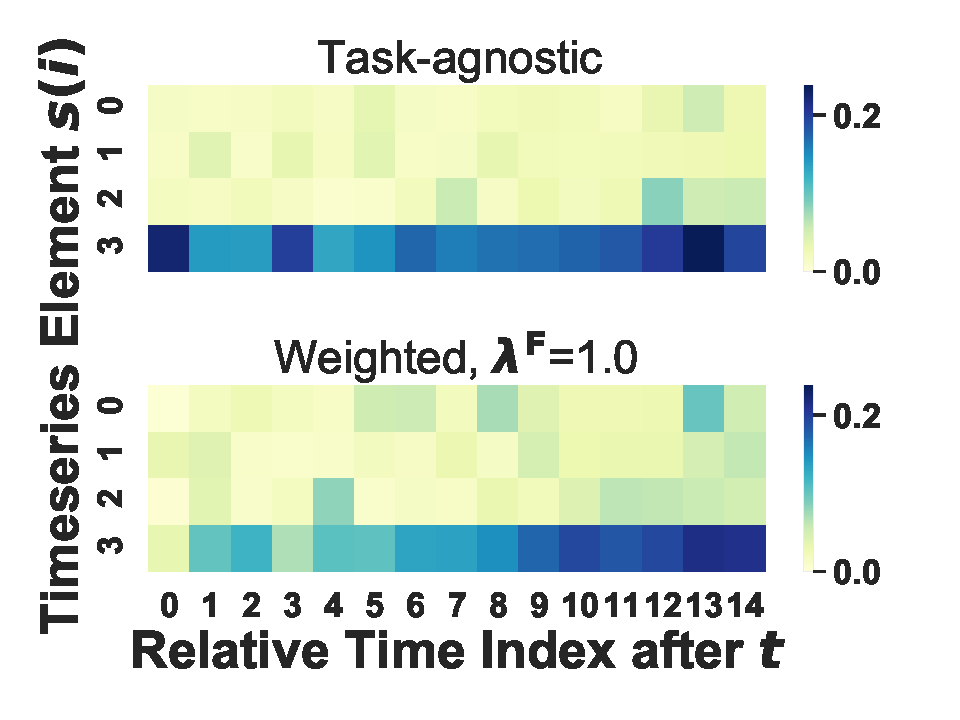
\includegraphics[width=0.31\columnwidth]{figures/iot/forecast_errors.pdf}}
\label{fig_iot_forecast_errors}
}
%\subfigure[]{
\subfigure{
{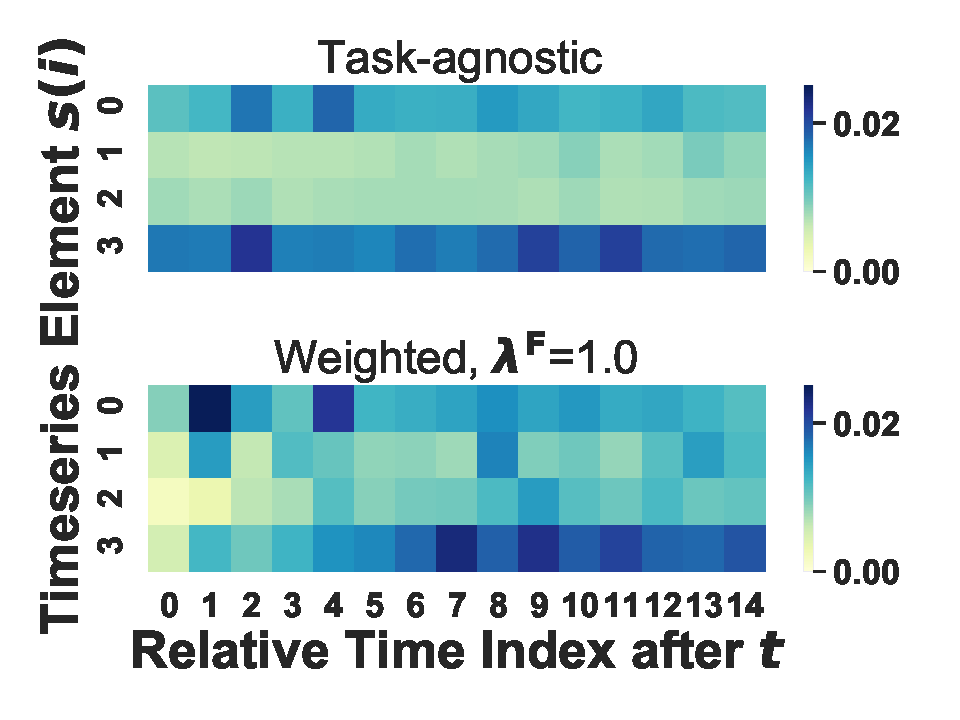
\includegraphics[width=0.31\columnwidth]{figures/cell/forecast_errors.pdf}}
\label{fig_cell_forecast_errors}
}
%\subfigure[]{
\subfigure{
{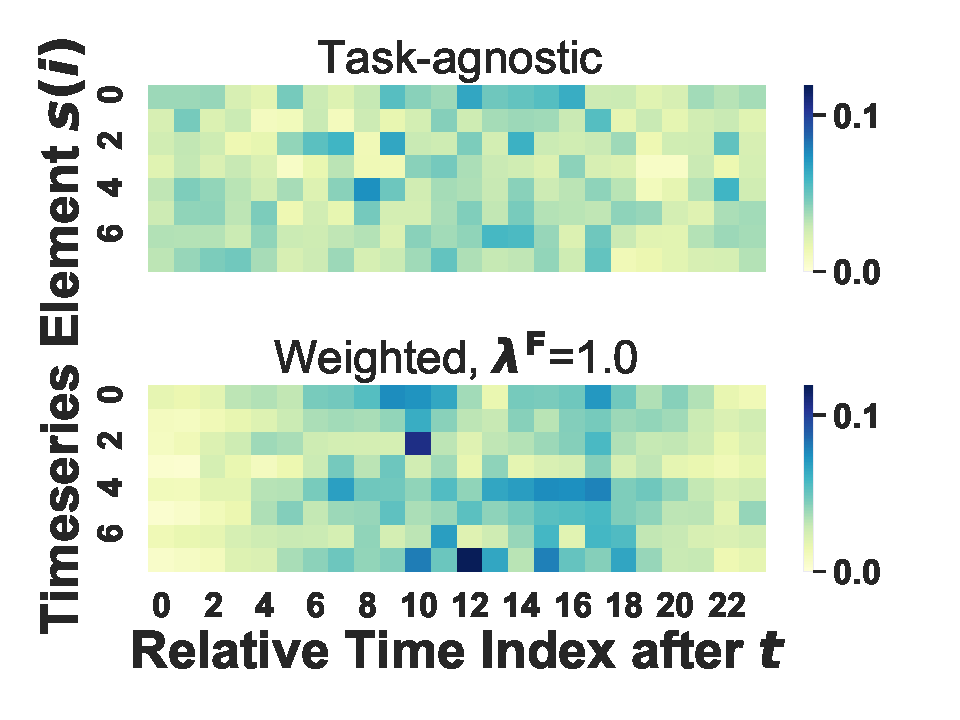
\includegraphics[width=0.31\columnwidth]{figures/pjm/forecast_errors.pdf}}
\label{fig_pjm_forecast_errors}
}
\caption{\textbf{Forecasting error comparison: task-agnostic vs. weighted scheme.} From left to right, the columns correspond to smart factory regulation from IoT sensors, taxi dispatching with cell demand, and battery storage optimization. The heatmaps show how co-design minimizes errors on timeseries elements $s(i)$ and forecast horizons that are salient for the control task when $Z=3$.}
\label{fig_heatmap}
\end{center}
\vskip -0.2in
\end{figure*}
%Aggregated forecasting error for  each relative time index when $Z=3$, under different policies. (j-l) Forecasting error for each $s(i)$ and each relative time index when $Z=3$, under task-agnostic (top) and weighted (bottom) policy, respectively.
%\caption{Results for real data. Columns from left to right corresponds to smart home regulation, taxi dispatching and battery storage optimization, respectively. (a-c) Control cost $J$ under different bottleneck dimension $Z$ and training policies; (d-f) Control error for each $u(i)$ when $Z=3$ under different training policies; (g-i) Aggregated forecasting error for  each relative time index when $Z=3$, under different policies. (j-l) Forecasting error for each $s(i)$ and each relative time index when $Z=3$, under task-agnostic (top) and weighted (bottom) policy, respectively.}
